%%%%%%%%%%%%%%%%%%%%%%%%%%%%%%%%%%%%%%%%
%%%%%  Chapitre Histoire
%%%%%%%%%%%%%%%%%%%%%%%%%%%%%%%%%%%%%%%%

\chapter{Une histoire de fous}
\mtcaddchapter

\section{Au commencement était \TeX} \index[con]{tex@\TeX!histoire}

\TeX\ (du grec $\tau \epsilon \chi$ qui a donné le mot \og technique \fg{} et qui explique la prononciation \og tèque \fg{}) est un programme de mise en forme de textes techniques, du simple article aux ouvrages en plusieurs tomes. Pour mieux comprendre l'aspect quasi-légendaire de \TeX, un peu d'histoire. 


\subsection{Le contexte}

Durant les années 70, Donald E. \textsc{Knuth}\cite{knut}, un mathématicien américain, s'était attelé à l'écriture de ce qui est désormais une référence fondamentale (rien de moins) en informatique : \emph{The Art of Computer Programming}. Dès l'origine, il avait planifié la sortie de plusieurs volumes sur une quarantaine d'années ! Or, en 1977, Donald \textsc{Knuth} rencontra un problème très particulier\footnote{Ce texte, maladroitement traduit par votre serviteur, a pour une source une conférence de Donald \textsc{Knuth} en 1986, reprise \emph{in extenso} dans le \href{http://www.tug.org/TUGboat/Contents/contents7-2.html}{septième numéro} de la revue TUGboat, page 95--98. \`{A} l'adresse \liensimple{ http://www.webofstories.com/play/17110?o=MS} se trouve une interview vidéo de Donald \textsc{Knuth} sur ce thème.}.

\begin{quotation} %\piccaption{Donald \textsc{Knuth}}
\parpic[r]{\fbox{\resizebox{3cm}{!}{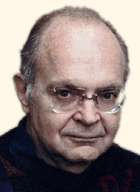
\includegraphics{images/Knuth.jpg}}}}\label{photoknuth} \og \emph{Pourquoi ai-je commencé à écrire \TeX\ en 1977 ? Cette histoire avait débuté longtemps auparavant, à l'occasion de la publication de mes livres \emph{The Art of Computer Programming}. J'avais préparé une seconde édition du tome 2, mais lorsque je reçus les épreuves, ce fut horrible --- la technique d'impression avait radicalement changé depuis la première édition. Les livres étaient maintenant composés à l'aide de photocomposeuses, au lieu des monotypes à plomb fondu ; en outre (hélas !), ces photocomposeuses étaient pilotées par des ordinateurs au lieu d'être supervisées \og manuellement \fg{}. Il en résultait une gestion désastreuse des blancs, surtout quand il s'agissait de mathématiques, et les fontes étaient décevantes comparées aux anciennes.} 

\emph{J'étais désespéré et ne savais que faire. \emph{Addisson-Wesley}\footnote{\'{E}diteur spécialisé dans les domaines scientifiques.} m'offrit de tout recomposer à l'aide des vieilles monotypes, mais je savais que la vieille méthode de composition était en train de mourir rapidement ; j'étais certain que lorsque j'aurai fini le tome 4, le même phénomène se reproduirait de nouveau et je ne voulais pas d'un résultat qui ressemblerait aux épreuves que j'avais vues. (...)} 
\end{quotation}

\begin{quotation}
\emph{Dès son début, en 1977, le projet de recherche \TeX\ dans lequel j'étais embarqué comportait deux axes principaux. Le premier était la qualité : nous ne voulions pas produire de bons documents, nous voulions qu'ils soient les meilleurs. (...)} 

\emph{Le second but recherché était l'archivage : il s'agissait de créer un système qui serait indépendant, autant que faire se peut, des mutations technologiques. Lorsqu'une nouvelle génération de machine à imprimer arriverait, je voulais être capable de maintenir le même niveau de qualité au lieu de repartir à zéro. Je voulais produire quelque chose qui pourrait encore servir dans un siècle. En d'autres termes, mon but était de m'y prendre de telle manière que, si l'on sauvegardait les spécifications d'un livre, nos descendants seraient encore capables d'éditer le même livre en l'an 2086.} \fg{}
\end{quotation}


\subsection{Le résultat}

La première version de \TeX\ date de 1978. Suite à corrections d'erreurs et à quelques évolutions, Donald \textsc{Knuth} décida de figer \TeX\ en 1982 à la version 3.14159\footnote{Chaque nouvelle version de \TeX\ ajoute des décimales de $\pi$ au numéro de version.}. 

En terme de qualité et conformément à l'idée initiale, \TeX\ a de quoi surprendre. Ainsi, son unité de longueur de référence la plus petite, le \emph{scaled point}, équivaut à $5,4\times10^{-9}$m. Autrement dit, les caractères sont ici placés avec une précision dépassant largement la précision de l'\oe il humain puisque nous nous plaçons ici à une échelle de l'ordre de grandeur du spectre de la lumière visible. \TeX\ sera donc dépassé quand l'évolution nous aura fait nous passer de nos yeux !

En terme informatique, \TeX\ est à la fois un programme et un langage. \TeX\ est ainsi un programme convertissant un fichier texte en un document décrivant la manière de positionner et de présenter ce texte sur une suite de pages. Par ailleurs, \TeX\ est un langage composé de plus de 300 fonctions dites \og primitives \fg{}. Ces fonctions, placées dans le fichier texte, permettent d'indiquer au programme \TeX\ comment présenter le texte. 

Ces fonctions, généralement simples, ont le désavantage de ne pas permettre de traiter un texte aisément. Seule l'action consécutive de plusieurs d'entre elles permet d'obtenir des résultats complexes, mais naturels. Ainsi en est-il, par exemple, de la création d'une page titre : dans ce cas, le texte sera centré selon plusieurs critères (le format de la page en particulier), sera écrit plus grand, sera sur une feuille séparée des autres, feuille qui ne sera pas numérotée... De fait, \TeX\ permet de créer une nouvelle fonction de présentation par composition de fonctions primitives : une \terme{macrocommande} ou macros, nommées dans toute la suite commandes. Bien entendu, de nouvelles commandes peuvent également s'obtenir par composition de commandes existantes.

Un ensemble de commandes pensées pour permettre de présenter un document forme un sur-ensemble de \TeX, un \terme{format}. Le premier format créé par \textsc{Knuth}, un format minimal, s'appelle \emph{plain}.  


\section{Puis vint \LaTeX}

\parpic[r]{\fbox{\resizebox{3cm}{!}{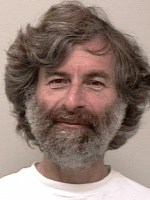
\includegraphics{images/Lamport.jpg}}}}
\LaTeX\ (prononcé \og latèque \fg{}), écrit en 1982 par Leslie \textsc{Lamport} \cite{lamp}, est un format simplifiant l'usage de \TeX\ en le dotant de commandes exécutant des tâches importantes de présentation. 

Par la suite, des ensembles de commandes ont été développés, ceci afin de développer tel ou tel aspect particulier de présentation : par exemple offrir des mises en page alternatives des titres. Un tel ensemble de commandes regroupées en un fichier est ici appelé une \terme{extension} ou un \og \terme{paquet} \fg{} (en anglais \emph{package}). 

Et les besoins d'extension étaient vastes ! Les possibilités de \TeX\ par le biais de \LaTeX\ et de ses extensions ont, de fait, explosé. D'un logiciel pensé pour écrire des articles scientifiques assez stéréotypés, \TeX\ est devenu un logiciel pensé pour rédiger des documents très variés --- de la simple lettre au livre en passant par les transparents ou des partitions --- dans des domaines aussi différents que la physique, la chimie, les mathématiques, la linguistique, la musique, le jeu d'échecs, etc. 

Depuis 1994, la version normalisée s'appelle \LaTeXe{} (qui se lit \og latèque deux oeufs \fg{}). Elle est compatible (dans la mesure du possible) avec les anciens standards.


\section{Longtemps après vinrent \XeTeXtitre et \XeLaTeXtitre}

\parpic[r]{\fbox{\resizebox{3cm}{!}{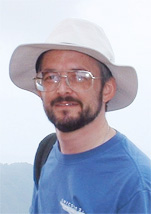
\includegraphics{images/Kew.jpg}}}}
\TeX\ et \LaTeX\ sont rapidement devenus des outils internationaux mais ils avaient quelques limitations, en particulier sur la gestion de langues étrangères et de polices de caractères. Ceci s'expliquait en particulier par une problématique d'encodage que Jonathan \textsc{Kew}, avec \XeTeX, fit grandement avancer.

Fondamentalement, les ordinateurs ne traitent que des nombres binai\-res. Un fichier texte ne contient pour ainsi dire qu'une chaîne de zéros et de uns. Pour que l'ordinateur nous restitue des caractères, il faut avoir recours à un \terme{encodage} autrement dit une table de correspondance qui permet de dire que telle chaîne binaire est associée à tel caractère unique. Par exemple, en encodage ASCII, \og 01000001 \fg{} correspond à la lettre \og A \fg{}. 

Cependant, il existe plusieurs encodages et ils ne sont pas forcément cohérents entre eux. Depuis 1991, un projet d'encodage mondial suit cependant son cours : Unicode\footnote{Le site officiel d'Unicode présente très largement cet encodage : \liensimple{http://www.unicode.org/}.}. Il a pour but de traiter les différents langues de l'humanité en un unique encodage : s'y retrouvent des langues aussi variées que le japonais, le tamul, le tagalog, le khmer.% de fait, des caractères aussi différents que ȹ, Җ, څ , ௸, ⾦. 

Du fait de ses travaux l'amenant à travailler avec des langues asiatiques, Jonathan \textsc{Kew}\footnote{Une interview de Jonathan \textsc{Kew} sur ce sujet : \liensimple{http://tug.org/interviews/kew.html}.} proposa en 2004 une version de \TeX, nommée \XeTeX\ (prononcé \og zétex\fg), permettant de gérer l'Unicode et donc le multilinguisme.

\XeTeX\ et \paquet{fontspec} --- un paquet dédié à la gestion des polices de caractères --- offrent en plus des fonctionnalités plus étendues (voir page~\pageref{fontes}) :
\begin{itemize}
\item accès généralisé aux polices OpenType Fonts (OTF) et TrueType Fonts (TTF) ;
\item accès à des caractères alternatifs et à des ligatures spécifiques de ces polices ;
\item gestion de la transparence des caractères ;
\item simplification de la chaîne de compilation pour \paquet{pstricks}.
\end{itemize}

\section{Et \LuaTeXtitre et \LuaLaTeXtitre les rejoignirent}

Développé par Taco \textsc{Hoekwater}, Hartmut \textsc{Henkel} et Hans \textsc{Hagen}, \LuaTeX\footnote{Le site officiel est à l'adresse \liensimple{http://luatex.org/}.} étend les possibilités du monde \TeX\ dans une nouvelle direction : intégrer un langage de script, Lua, dans le code \TeX. Ceci permet de faire exécuter à \LaTeX\ par le biais de Lua des tâches plus complexes dans le traitement du texte : Lua peut en effet modifier le comportement de \TeX\ ou le compléter. De façon similaire, ceci permet de faire des calculs complexes avec \TeX, ce dernier étant relativement limité en ce domaine.

\section{Un souci}

L'actuelle variété du monde de \TeX\ a tout de même un prix dans la mesure où ces extensions et différentes versions de \TeX\ ont introduit des incompatibilités : différents paquets utilisent des noms de commandes identiques pour réaliser des tâches bien différentes. Du coup, une certaine prudence reste parfois de mise si de multiples paquets sont utilisés, ceci pour éviter des résultats erronés. 

Cette situation a conduit au projet de normalisation \LaTeX3, sous la direction des \og gurus \fg{} \LaTeX\ parmi lesquels se trouve Leslie \textsc{Lamport}\footnote{Pour plus de détails, consulter \liensimple{http://www.latex-project.org}.}. L'histoire n'a donc pas fini de se poursuivre !


\begin{flushright}
Vous cernez mieux la bête ? Passons alors à la \TeX nique !
\end{flushright}